\section{Segmentation}
This section will go through how the segmentation of the sound was achieved. The segmentation is needed to locate each sound's endpoints in a signal, i.e. the positions in time at which each sound starts and ends. This is a necessary part of the transcription system as we need to be able to distinct the sounds from each other and not the whole signal as a combination of many sounds.

In this transcription system the segmentation is made by calculating the logarithm of the RMS of each window and if this value, from one window to the next, goes above a threshold it is considered as the starting point of a sound. Similarly when the value falls below the threshold the end of the sound is registered.

The Matlab function for segmenting the signal analyses the signal using a specified window size and window skip. When all endpoints in the signal are found, a cell array is returned containing the signal divided into segments so that each cell contains the frames for that segment.

\begin{figure}[h]
	\begin{center}
		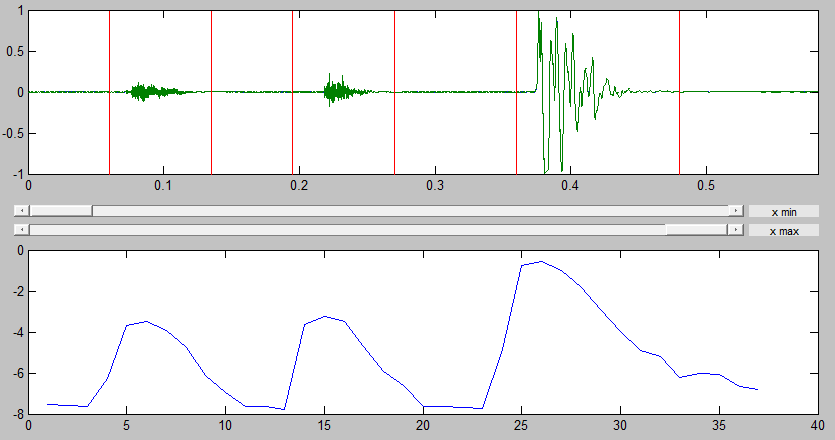
\includegraphics[scale =  0.4]{fig/SegmentationPic.png}
		\caption{An example of how the signal will be segmented. On the top the signal is plotted in the time domain with vertical lines indicating the segmentation points (endpoints). The bottom shows the logarithm of the RMS to the signal from above}
		\label{SegmentationPic}
	\end{center}
\end{figure}

An example of the result from this segmentation is shown in figure \ref{SegmentationPic}. At the top we see the input signal and vertical lines indicating the endpoints of each segment. On the bottom of the figure a graph of the change in the logarithm of the RMS is plotted where we see a peak at each segment in the signal.